\scanpage{8}
\mspage{2}
We have a bijective map.
\[
\vec A\overset{\mathrm{rd}}{\simeq}A_{\unsure{*|\leftarrow|+}}(C)\quad\text{set of edges of }C
\]
\[
\vec a\longmapsto\text{``\deleted{\unsure{left}}\inserted{right} bank of $\unsure{-|\vec a}$''}
\]
and each edge of $C$ is oriented in a natural way via this map. Thus the set of \uline{arcs} $\vec A(C)$ is identified:
\[
A(C)\times\{\pm1\}\simeq\vec A\times\{\pm1\},
\]
and the map $\sigma_0^C$ (passage to \unsure{the other|the edge} opposite) is identified: $\deleted{\unsure{\sigma}}\unsure{\sigma_\Gamma|\mathrm{id}|\sigma_0}\times\tau$, $\tau$ the transposition of $\pm1$. Remains: to define $\sigma_1^C$, we define it separately on
\[
\underbrace{\vec A\times\{+1\}}_{=\uline{\mathrm{rg}(\vec A)}}=\vec A(C)_+
\]
and on
\[
\underbrace{\vec A\times\{-1\}}_{\mathrm{rd}(\vec A)}=\vec A(C)_-.
\]
We have:
\margin{\uline{NB} $\vec A(C)_+$ is an \uline{orientation} of the contours}
\figure{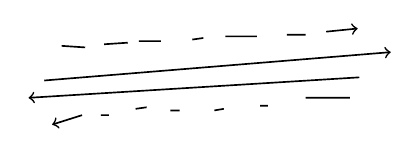
\begin{tikzpicture}[x=.02cm,y=-.02cm,line width=.6pt]
\draw[->] (115,705)--(335,687);
\draw[->] (315,703)--(105,716);
\draw (126,683)--(141,684) (153,682)--(168,681) (175,680)--(189,680) (209,679)--(216,678) (230,677)--(250,677) (269,676)--(281,676);
\draw[->] (294,674)--(314,672);
\draw[<-] (120,733)--(139,727);
\draw (151,727)--(156,727) (173,723)--(180,722) (195,724)--(201,724) (223,724)--(229,723) (252,721)--(257,721) (281,716)--(309,716);
\end{tikzpicture}}
\figure{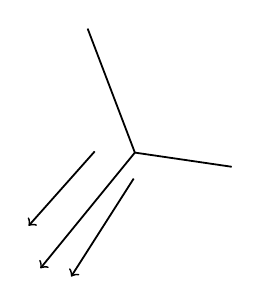
\begin{tikzpicture}[x=.015cm,y=-.015cm,line width=.65pt]
\draw (145,969)--(185,1074)--(267,1086);
\draw[->] (185,1074)--(105,1172);
\draw[->] (151,1073)--(95,1136);
\draw[->] (184,1096)--(131,1179);
\end{tikzpicture}}
\margin{$A$}
\figure{\begin{tikzpicture}
\node[inner sep=3pt] (f) {$\displaystyle
\left\{\begin{aligned}
\sigma_1^C(\mathrm r\deleted{\unsure{\mathrm g}}\mathrm d(\vec a))&=\deleted{\unsure{\mathrm{rd}}}\mathrm{rg}(\rho_\Gamma^{-1}(\vec a))=\sigma_0^C\mathrm{rd}(\rho_\Gamma(\vec a))\\
\sigma_1(\mathrm r\deleted{\unsure{\mathrm d}}\mathrm g(\vec a))&=\mathrm r\deleted{\unsure{\mathrm g}}\mathrm d(\rho_\Gamma^{\deleted{\unsure{-1}}}(\vec a))\deleted{\unsure{=\sigma_0^C}}
\end{aligned}\right.$};
\draw ([xshift=3pt,yshift=7pt]f.north west)--([xshift=7pt,yshift=7pt]f.north east);
\draw[->] ([xshift=7pt,yshift=7pt]f.north east)--([xshift=3pt]f.east);
\draw ([xshift=3pt,yshift=-1pt]f.east)--([xshift=3pt,yshift=-5pt]f.south east);
\draw ([xshift=1pt,yshift=-5pt]f.south east)--([xshift=-6pt,yshift=-5pt]f.south west)--([xshift=-6pt,yshift=1pt]f.north west);
\end{tikzpicture}}
\[
\Longrightarrow\quad\cdot\quad
\deleted{\rho_s(\vec a)=}
\left\{\begin{aligned}
\rho_C(\mathrm{rd}\vec a)&=\mathrm{rd}(\rho_\Gamma^{\deleted{\unsure{-1}}}(\vec a))\\
\rho_C(\mathrm{rg}\vec a)&=\mathrm{rg}(\rho_\Gamma^{-1}\deleted{\unsure{\sigma_\Gamma}}\vec a))
\end{aligned}\right.
\]
\margin{\uline{NB} \inserted{The definition} of the \uline{oriented} \uline{contours} $C$ depends only on $\vec A$ equipped with $\rho_\Gamma$ (to the exclusion of $\sigma_0$)}

\unsure{The} contour $C$ : \unsure{incident} \unsure{sense} of the \unsure{Aristyp.}

a) $C$ is oriented (``\unsure{positive|obvious} direction around $\Gamma$'')
\deleted{\deleted{\unsure{C|the}} \deleted{\unsure{A|C}} $C'$ by ``juxtaposition'' i.e. each \inserted{(takes account of $\unsure{o}$)} \unsure{edge|is} \unsure{is} \unsure{oriented}, that is the datum of a \unsure{canonical} map}
\[
\deleted{\vec A(C)'_+\subset\vec A(C),}
\]
\deleted{(``\unsure{topological} \unsure{regions}'') : the \unsure{unique} p.}
\[
\deleted{A(C)\longrightarrow\pm1}
\]
\deleted{\unsure{giving} the value \unsure{$+1$ and $-1$} on the two \unsure{sides}.}

\margin{i.e. we have ---\par
$\vec A=\vec A(C)_+\subset\vec A(C)$\par
or\par
$\sigma_0\vec A=\vec A(C)_-\unsure{\sim\vec A|\simeq\vec A|\deleted{\sim\vec A}|\deleted{\simeq\vec A}}$\par
$\sigma_1\vec A=\vec A(C)_-\unsure{\sim\vec A|\simeq\vec A|\deleted{\sim\vec A}|\deleted{\simeq\vec A}}$}
Thus
\[
\left\{\begin{aligned}
\vec A(C)&\simeq\uline{\vec A(C)_+}\times\{\pm1\},\\
\sigma_0^C&\simeq\mathrm{id}\times\tau
\end{aligned}\right.
\]
The datum of $\sigma_1^C$ amounts to that of a permutation
\[
\rho_C^{\unsure{\bullet}}=\hookleftarrow\{\vec a\longrightarrow\sigma_1^C(\sigma_0^C(\vec a)))\quad\text{on }\vec A
\]
b) We have an involution, without fixed points \inserted{$\sigma_{\unsure{0|\Gamma}}^C$} on the set \deleted{\unsure{of the}} of the sides of $\unsure{\Delta|C}$, which is identified:
\[
\vec A=\vec A(C)_+.
\]
\margin{7}
